\documentclass{beamer}

\usepackage[english]{babel}
\usepackage[T1]{fontenc}
\usepackage[utf8]{inputenc}

\usepackage{fancyvrb}
\usepackage{enumitem}

% Règle les conflits beamer/enumitem
\setitemize{label=\usebeamerfont*{itemize item}
\usebeamercolor[fg]{itemize item}
\usebeamertemplate{itemize item}}

\usetheme{Antibes}
\title{M2M - 2016 - RDSMining}
\graphicspath{{imgs/}}
\author{Ronan ABHAMON \\~ Florian BIGARD}
\institute{Université Joseph Fourier}
\date{\today}

\setbeamertemplate{itemize item}[triangle]

% A chaque changement de section, affichage de la section dans une diapo
\AtBeginSection[ ]
{
	\begin{frame}
 		\tableofcontents[currentsection,hideothersubsections]
 	\end{frame}
}

% Marges du diapo
\setbeamersize{text margin left=0.8cm, text margin right=0.8cm}

% Numéros de pages
\defbeamertemplate*{footline}{shadow theme}
{
	\leavevmode
	\hbox{\begin{beamercolorbox}[wd=1.0\paperwidth,ht=2.5ex,dp=1.125ex,leftskip=.3cm plus1fil,rightskip=.3cm]{author in head/foot}
    	\usebeamerfont{author in head/foot}\insertframenumber\,/\,\inserttotalframenumber\hfill
	\end{beamercolorbox}
}
	\vskip0pt
}

\begin{document}

\begin{frame}
	\titlepage
\end{frame}

\section{Architecture}
\begin{frame}
	\begin{center}
		\includegraphics[scale=0.38]{architecture.png}
	\end{center}
\end{frame}

\section{Beagleboard black}

\subsection{FM-Tuner Service}

\begin{frame}[fragile]
	\begin{block}{FM-Tuner Service}
		\begin{itemize}
			\item A high level si4703 service (C gnu99 program).
			\item Working on a single thread (RDS parser + server).
			\item Non-blocking I/O.
			\item Working with systemd.
			\item Send changes/notifications to clients.
		\end{itemize}
	\end{block}
	\begin{block}{Messages}
		\begin{itemize}
			\item A specific protocol working in TCP:
		\end{itemize}
		\begin{center}
			\begin{minipage}{10cm}
				\begin{verbatim}
LENGTH TYPE_1 VALUE_1 [TYPE_N VALUE_N...]
				\end{verbatim}
			\end{minipage}
		\end{center}
	\end{block}
\end{frame}

\subsection{FM-Tuner Message Broker}

\begin{frame}
	\begin{block}{FM-Tuner Message Broker}
		\begin{itemize}
			\item A simple broker. (nodeJS program, ES7)
			\item Set the channel/volume. (Send message to service)
			\item Print service notifications.
			\item Send by MQTT the radio name.
		\end{itemize}
	\end{block}
\end{frame}

\section{Server}

\subsection{ElasticSearch}

\begin{frame}
	\begin{center}
		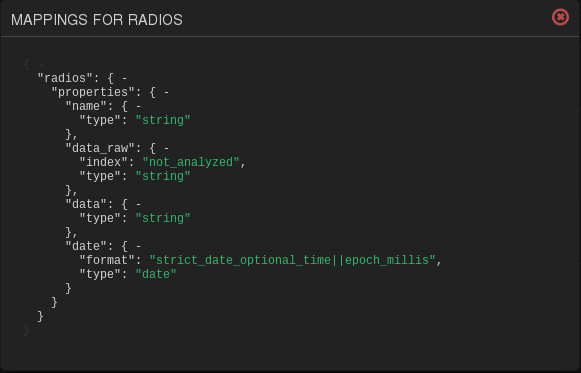
\includegraphics[scale=0.50]{mapping.png}
	\end{center}
\end{frame}

\subsection{Kibana}

\begin{frame}
	\begin{center}
		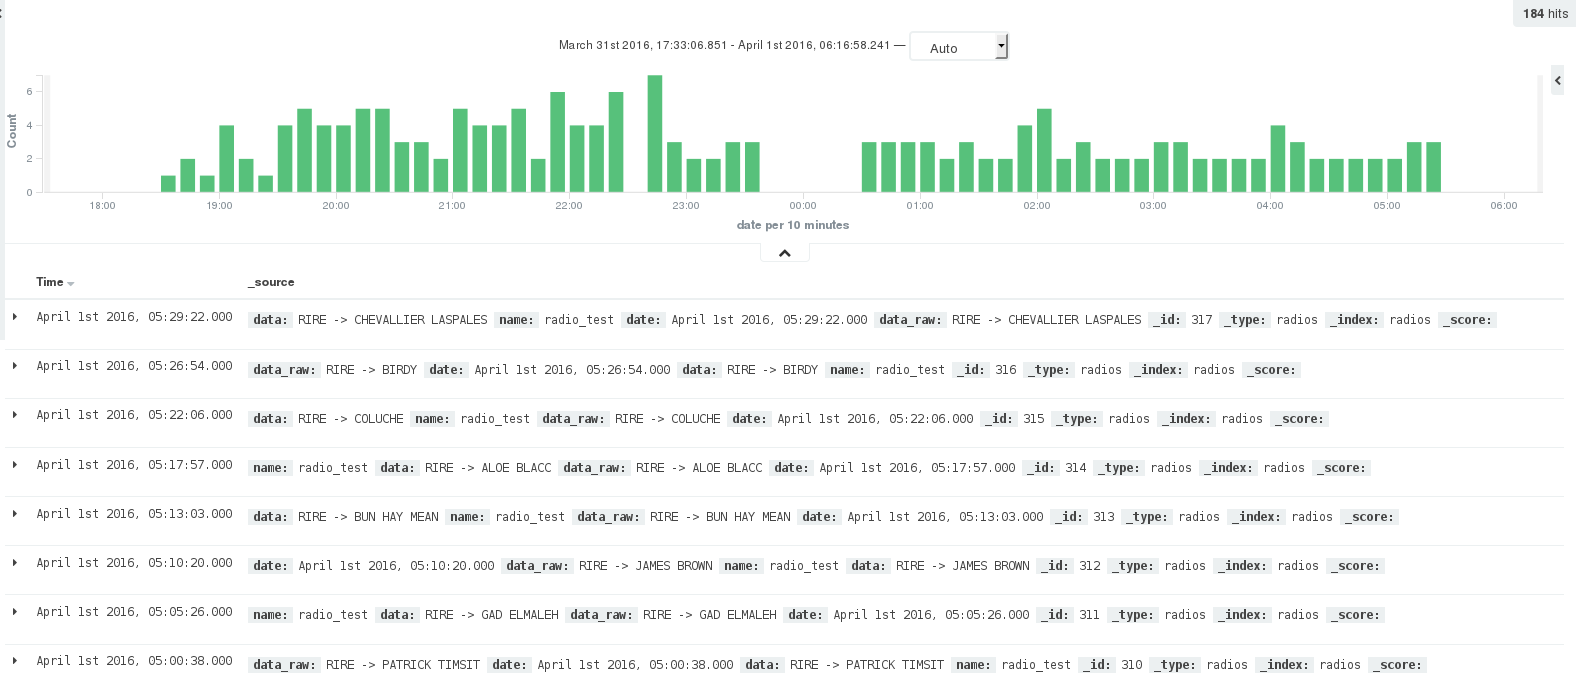
\includegraphics[scale=0.20]{frequence.png}
	\end{center}
\end{frame}

\end{document}
